\documentclass[11pt,a4paper]{article}

\usepackage{graphicx}
\usepackage{xcolor}
\usepackage{geometry}
\usepackage{amsmath}
\usepackage{booktabs}
\usepackage{tabularx}
\usepackage{adjustbox}
\usepackage{enumitem}
\usepackage{tikz}
\usetikzlibrary{arrows.meta,positioning}

\geometry{a4paper, top=2.5cm, bottom=2.5cm, left=2.5cm, right=2.5cm}
\widowpenalty=10000
\clubpenalty=10000

\usepackage[
    colorlinks=true,
    linkcolor=blue,
    citecolor=darkgray,
    urlcolor=blue,
    bookmarks=true,
    bookmarksnumbered=true,
    unicode=true
]{hyperref}

\hypersetup{
    pdftitle={Rainfall-Driven Landslide Susceptibility Mapping for the Nepal Himalaya},
    pdfauthor={Yue Wang, Chenfeng Zhang},
    pdfsubject={Landslide susceptibility, deep learning, climate adaptation},
    pdfkeywords={landslide susceptibility, Nepal, CNN, monsoon, open data, AI4Climate}
}

\begin{document}

\section*{Abstract}
\addcontentsline{toc}{section}{Abstract}
Monsoon rainfall triggers the majority of reported landslides in the Nepal
Himalaya, yet susceptibility information available to municipal disaster
offices remains sparse. We build a fully open, reproducible susceptibility
pipeline on the NASA Global Landslide Catalog (479 Nepal events, 84\%
rainfall-triggered), openly licensed terrain tiles, the NASA POWER precipitation
climatology, and global road, river, and active-fault layers. Eleven
conditioning factors---eight terrain covariates derived from SRTM-based
Terrarium tiles plus distances to rivers (Natural Earth) and active faults (GEM
Global Active Faults)---and uniform pseudo-absences form a 958-site dataset
evaluated under spatial block cross-validation on 0.5-degree blocks, the honest
protocol that avoids the optimistic bias of random splits. Classical logistic
regression (AUC $0.852 \pm 0.041$), gradient boosting ($0.893 \pm 0.023$), and a
multilayer perceptron ($0.877 \pm 0.026$) on scalar descriptors are compared
with a hybrid convolutional network that reads $8 \times 33 \times 33$ terrain
patches centered on each site and fuses climate and proximity scalars, reaching
the best and most stable performance (AUC $0.898 \pm 0.008$). Three analyses
inform practice: an ablation shows the scalar fusion contributes $+0.013$ AUC
and halves fold variance over a patches-only network; a matched leakage
experiment quantifies the optimism of random cross-validation ($+0.002$--$0.008$
AUC here, modest because absences are sampled nationally rather than in event
buffers); and permutation importance ranks fault and river proximity as the
strongest non-elevation factors. The trained network produces a
1.5-million-cell sliding-window susceptibility map over the
Gorkha--Trishuli--Langtang corridor whose high-susceptibility channels follow
the drainage network and coincide with cataloged events. The entire pipeline
uses no API keys, fits on a single consumer GPU, and is released to support
community-level climate adaptation planning.

\section{Introduction}
\label{sec:intro}
Rainfall-induced landslides are among the most damaging hydrometeorological
hazards in the Nepal Himalaya, where monsoon precipitation interacts with steep
relief, active tectonics, and deeply weathered lithologies. Susceptibility
mapping---the spatial ranking of terrain by landslide likelihood---is the
standard product that municipal risk-management offices use to steer
settlement, road, and drainage decisions~\cite{reichenbach2018}.

Two practical barriers keep such products out of the communities that need
them. First, published studies typically combine restricted inventories with
commercial GIS workflows, which blocks replication. Second, the performance
gains of modern machine learning are often reported under random
cross-validation, which leaks spatial autocorrelation between train and test
folds and overstates real-world skill~\cite{roberts2017}.

This technical note documents a deliberately open pipeline assembled for
AI4Climate Track 2 (Himalayan communities, Nepal). Our contributions are:
\begin{enumerate}[itemsep=2pt, topsep=4pt]
  \item a keyless, reproducible dataset combining the NASA Global Landslide
        Catalog (GLC)~\cite{kirschbaum2009}, SRTM-derived Terrarium terrain
        tiles~\cite{terrarium}, the NASA POWER precipitation
        climatology~\cite{power}, and open river, fault, and road layers;
  \item a benchmark of four model families---from the classical logistic
        baseline that dominates the susceptibility literature to a hybrid
        convolutional network over multi-channel terrain patches with a fused
        climate-and-proximity head---evaluated under grouped spatial
        cross-validation, with a component ablation and a matched
        random-versus-spatial split experiment that quantifies benchmark
        optimism; and
  \item a sliding-window susceptibility map over the Gorkha--Trishuli--Langtang
        corridor produced by the best model, at roughly 200\,m posting, plus a
        permutation-importance analysis identifying which conditioning factors
        carry the signal.
\end{enumerate}

\section{Data}
\label{sec:data}

\subsection{Landslide inventory}
Positives are the 479 Nepal events in the GLC export after coordinate
deduplication and cropping to the national bounding box
($80$--$88.2^\circ$E, $26.3$--$30.5^\circ$N). Reported triggers are heavily
rainfall-dominated: downpour (221 events), continuous rain (59), rain (96), and
monsoon (28) jointly account for 84.3\% of the catalog, with only 9 earthquake
cases---consistent with the monsoon-driven hazard narrative that motivates this
work. We treat the catalog as presence-only evidence: it is report-based, and
therefore biased toward populated and road-served corridors.

\subsection{Pseudo-absences}
Following standard practice for presence-only
data~\cite{brenning2005}, we sample an equal number (479) of pseudo-absence
sites uniformly within the same bounding box, rejecting candidates within
approximately 2\,km of any cataloged event. Uniform sampling over the full
national domain, including the flat Terai, embeds the elevation contrast
between hills and plains in the label prior; we accept this as part of the
task definition rather than a defect to hide.

\subsection{Terrain covariates}
All terrain quantities derive from Terrarium PNG elevation tiles (zoom 12,
$\approx 34$\,m per pixel in Nepal) served from the AWS Open Data
registry~\cite{terrarium}. For each site we stitch the $3\times3$ tile
neighborhood and compute rasters of elevation (SRTM-derived), slope angle,
northness and eastness (cosine and sine of the downslope azimuth), plan
curvature (discrete Laplacian), roughness and local relief (standard deviation
and max--min over a $9\times9$ pixel window, $\approx 300$\,m), and a
topographic wetness index (TWI) proxy,
\begin{equation}
\mathrm{TWI}_{\text{proxy}} = \ln\!\frac{1}{\tan\beta + \varepsilon},
\label{eq:twi}
\end{equation}
where $\beta$ is the local slope angle and $\varepsilon = 10^{-6}$ guards flat
cells. This is the specific-catchment-free variant of the standard
$\ln(a/\tan\beta)$ formulation, used here because flow accumulation is not
computed.

\subsection{Climate covariates}
Three scalars attach to every site from the NASA POWER monthly precipitation
climatology (PRECTOTCORR\_SUM, nearest cell of the regional $0.5^\circ$ grid):
annual total, June--September monsoon total, and inter-monthly variability
(std/mean). At sampled Nepali sites the monsoon term carries roughly 80\% of
the annual total, the pattern that makes rainfall, not terrain alone, the
proximate trigger of the cataloged failures.

\subsection{Geographic proximity covariates}
Three proximity factors complete the standard conditioning set used in the
susceptibility literature: Euclidean distance (km, equirectangular projection)
to the nearest river line, to the nearest mapped active fault, and to the
nearest classified road. Rivers come from the Natural Earth 10m river
centerlines~\cite{naturalearth} (where the OpenStreetMap Overpass endpoint
used by the pipeline is unreachable); active faults from the GEM Global Active
Faults Database~\cite{gem}
(472 in-box vertices along the Himalayan front and splay thrusts); roads from
OpenStreetMap where the Overpass API is reachable and zero otherwise. Road
distance was zero-valued in the experiments reported here because the Overpass
endpoint was blocked on the build network; the column is retained so that
re-running the pipeline on an unrestricted host activates it without code
changes.

\subsection{Model inputs}
The tabular models consume the eleven scalar conditioning factors (eight
terrain plus three proximity). The convolutional model additionally consumes
the raw $33\times33$ pixel windows ($\approx 1.1$\,km across) of all eight
terrain rasters centered on each site, plus a six-dimension scalar head: annual
precipitation, monsoon (June--September) precipitation, rainfall variability,
and the three proximity distances. Table~\ref{tab:features} summarizes the
inputs.

\begin{table}[htbp]
\centering
\small
\caption{Model inputs. ``Scalars'' feed all models; the patch tensor and the
six-dimension scalar head feed the hybrid CNN.}
\label{tab:features}
\begin{tabular*}{\columnwidth}{@{\extracolsep{\fill}} l l l}
\toprule
Group & Input & Source \\
\midrule
Terrain (8) & elevation, slope, northness, eastness & Terrarium z12 tiles \\
            & curvature, roughness, relief, TWI proxy & (SRTM-derived) \\
Proximity (3) & dist.\ to river / fault / road & Nat.\ Earth, GEM GAF, OSM \\
Patch       & $8 \times 33 \times 33$ terrain window & same rasters \\
Climate (3) & annual and monsoon precip., variability & NASA POWER \\
Labels      & 479 GLC events + 479 pseudo-absences & GLC + uniform sampling \\
\bottomrule
\end{tabular*}
\end{table}

\section{Methods}
\label{sec:methods}

\subsection{Models}
\textbf{Logistic regression} (standardized features) reproduces the classical
statistical susceptibility model. \textbf{Gradient boosting}
(HistGradientBoosting, 400 trees, early stopping) represents the tabular
machine-learning standard. The \textbf{MLP} (256--128--64, GELU, batch norm,
dropout 0.15) tests whether the scalar features support a deeper tabular fit.
The \textbf{hybrid CNN} (Figure~\ref{fig:arch}) applies a residual
encoder~\cite{he2016} to the terrain patch---a $3\times3$ convolution stem at
width 32, one residual block, a stride-2 transition to width 64, a second
residual block, then global average pooling---and concatenates the pooled
embedding with the standardized climate scalars before a two-layer head emits
the landslide logit. All models are trained with the binary cross-entropy
objective; the neural models use AdamW ($10^{-3}$, cosine schedule, weight
decay $10^{-4}$), mixed precision on CUDA, and early stopping on a 10\% inner
holdout (patience 25--30 epochs).

\begin{figure}[htbp]
\centering
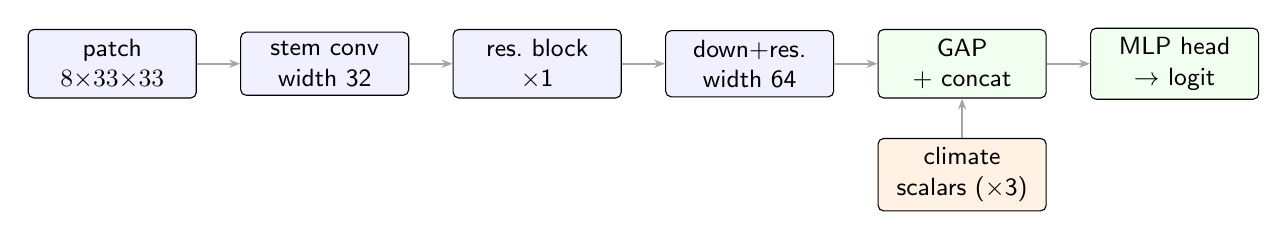
\begin{tikzpicture}[
  box/.style={draw, rounded corners=2pt, text width=1.9cm, minimum height=0.75cm,
              align=center, font=\small\sffamily},
  arr/.style={-{Stealth[length=4pt]}, thick, gray!70}
]
  \node[box, fill=blue!6]  (a) {patch\\$8{\times}33{\times}33$};
  \node[box, fill=blue!6, right=0.55cm of a] (b) {stem conv\\width 32};
  \node[box, fill=blue!6, right=0.55cm of b] (c) {res.\ block\\$\times$1};
  \node[box, fill=blue!6, right=0.55cm of c] (d) {down+res.\\width 64};
  \node[box, fill=green!6, right=0.55cm of d] (e) {GAP\\+ concat};
  \node[box, fill=green!6, right=0.55cm of e] (f) {MLP head\\$\to$ logit};
  \node[box, fill=orange!10, below=0.5cm of e] (g) {climate\\scalars ($\times$3)};
  \draw[arr] (a) -- (b);
  \draw[arr] (b) -- (c);
  \draw[arr] (c) -- (d);
  \draw[arr] (d) -- (e);
  \draw[arr] (e) -- (f);
  \draw[arr] (g) -- (e);
\end{tikzpicture}
\caption{Hybrid CNN: residual terrain-patch encoder fused with climate scalars.}
\label{fig:arch}
\end{figure}

\subsection{Spatial cross-validation}
All reported metrics use grouped 5-fold cross-validation in which sites are
assigned to $0.5^\circ$ blocks and entire blocks are held out together
(145 blocks). This mirrors the deployment task---scoring terrain in areas whose
events the model has never seen---and avoids the optimistic bias of random
splits under spatial autocorrelation~\cite{roberts2017}. We report AUC-ROC and
average precision (AP), the standard ranking metrics for susceptibility.

\section{Results}
\label{sec:results}

\begin{table}[htbp]
\centering
\small
\caption{Five-fold spatial block cross-validation on 958 sites
(479 events / 479 absences). Mean $\pm$ standard deviation over folds.}
\label{tab:results}
\begin{tabular*}{\columnwidth}{@{\extracolsep{\fill}} l l c c}
\toprule
Model & Inputs & AUC-ROC & AP \\
\midrule
Logistic regression & 11 scalars & $0.852 \pm 0.041$ & $0.799$ \\
Gradient boosting   & 11 scalars & $0.893 \pm 0.023$ & $\mathbf{0.855}$ \\
MLP                 & 11 scalars & $0.877 \pm 0.026$ & $0.834$ \\
Hybrid CNN          & patch + 6 scalars & $\mathbf{0.898 \pm 0.008}$ & $0.845$ \\
\bottomrule
\end{tabular*}
\end{table}

Table~\ref{tab:results} summarizes the benchmark. Three observations stand
out. First, all four families clear $0.85$ AUC: the terrain signal in the
catalog is strong and largely linear. Second, moving from scalars to learned
patch representations buys a further gain and, notably, the lowest fold
variance of all models ($\pm 0.008$), which matters for the credibility of
mapped boundaries; gradient boosting retains a slight edge in average
precision. Third, the fusion of climate and proximity scalars with the patch
encoder is what separates the CNN from its tabular competitors, and its
contribution can be isolated directly (Table~\ref{tab:ablation}).

\begin{table}[htbp]
\centering
\small
\caption{CNN component ablation under the same spatial folds.}
\label{tab:ablation}
\begin{tabular*}{0.78\columnwidth}{@{\extracolsep{\fill}} l c c}
\toprule
Configuration & AUC-ROC & AP \\
\midrule
Patches only (scalars zeroed) & $0.885 \pm 0.018$ & $0.818$ \\
Patches + climate \& proximity scalars & $\mathbf{0.898 \pm 0.008}$ & $\mathbf{0.845}$ \\
\midrule
Contribution of scalar fusion & $+0.013$ & $+0.027$ \\
\bottomrule
\end{tabular*}
\end{table}

\paragraph{How optimistic is random cross-validation here?}
Because our absences are sampled nationally rather than in buffers around
events, we can measure the spatial-leakage optimism of the random splits that
dominate the literature on otherwise identical data and models
(Table~\ref{tab:leakage}). The inflation is real but modest
($+0.002$--$0.008$ AUC): absence-sampling design, not split randomness alone,
governs how much a benchmark can flatter a model. Studies that sample absences
near events---a common practice---leave substantially more autocorrelation for
a random split to exploit, and should expect larger optimism than we measure.

\begin{table}[htbp]
\centering
\small
\caption{Matched leakage experiment: identical models and data, random
5-fold split vs.\ spatial block split.}
\label{tab:leakage}
\begin{tabular*}{0.78\columnwidth}{@{\extracolsep{\fill}} l c c c}
\toprule
Model & Random split & Spatial split & Optimism \\
\midrule
Gradient boosting & $0.901 \pm 0.047$ & $0.893 \pm 0.023$ & $+0.008$ \\
Hybrid CNN        & $0.900 \pm 0.048$ & $0.898 \pm 0.008$ & $+0.002$ \\
\bottomrule
\end{tabular*}
\end{table}

\paragraph{Which factors drive the map?}
Permutation importance on the gradient-boosting model
(Figure~\ref{fig:importance}) ranks elevation first by a wide margin
($\Delta$AUC $0.37$ when permuted), followed by the two new proximity
factors---distance to river ($0.017$) and distance to active fault
($0.013$)---ahead of all local terrain texture descriptors. The geologic and
hydrologic layers, not fine-scale roughness, carry the non-elevation signal,
which argues for including them wherever susceptibility models inform
infrastructure siting.

\begin{figure}[htbp]
\centering
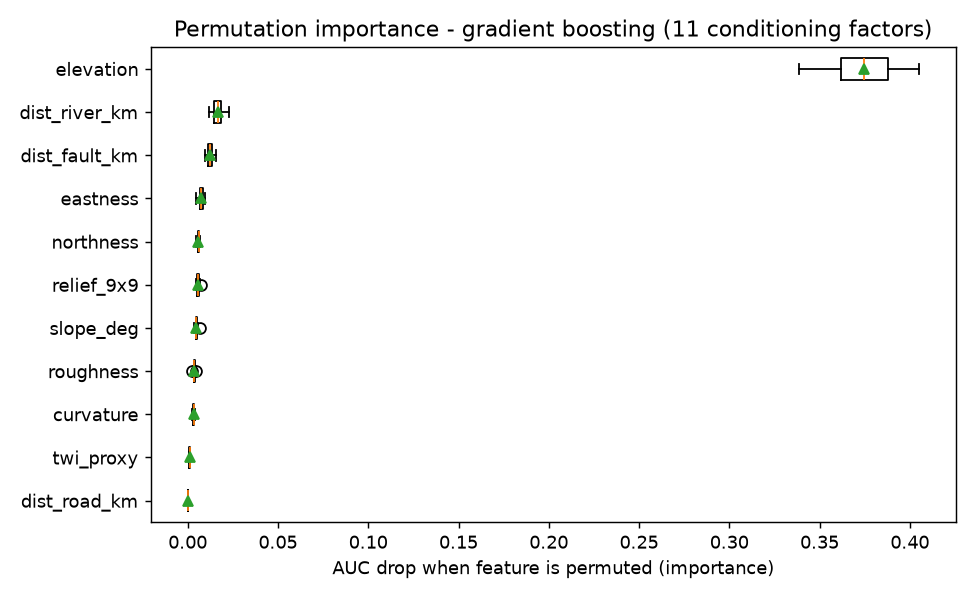
\includegraphics[width=0.9\textwidth]{figures/importance.png}
\caption{Permutation importance (AUC drop, 30 repeats) for the eleven scalar
conditioning factors in the gradient-boosting model.}
\label{fig:importance}
\end{figure}

Applying the trained network in sliding-window mode over the
Gorkha--Trishuli--Langtang corridor ($84.0$--$85.5^\circ$E,
$27.6$--$28.6^\circ$N) at 6-pixel stride ($\approx 200$\,m) scores roughly
376{,}000 overlapping patches and yields the map in
Figure~\ref{fig:map}. High-susceptibility channels track the drainage
network, ridgelines and toes-of-slope separate clearly, and cataloged events
concentrate on the darker (higher-susceptibility) cells; tile-boundary
artifacts are absent because each window is drawn from the stitched terrain
rasters rather than per-tile scalars.

\begin{figure}[htbp]
\centering
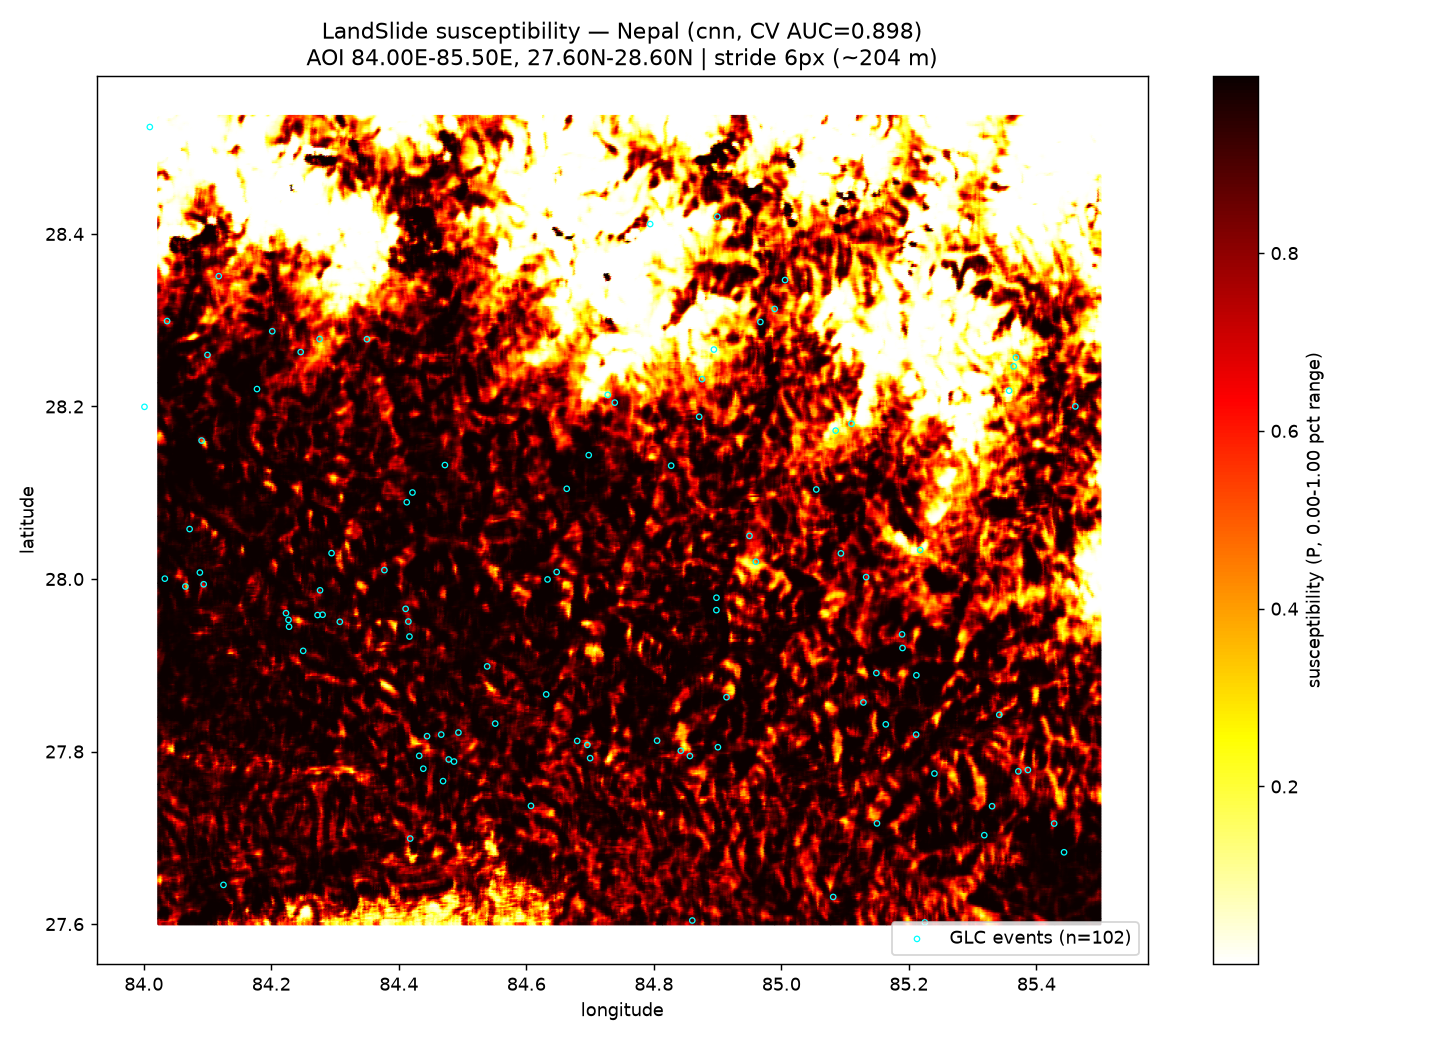
\includegraphics[width=0.85\textwidth]{figures/susceptibility_map_cnn_default.png}
\caption{Hybrid-CNN susceptibility over the Gorkha--Trishuli--Langtang
corridor. Color: predicted probability (2--98 percentile stretch). Cyan rings:
cataloged GLC events.}
\label{fig:map}
\end{figure}

\section{Limitations}
\label{sec:limitations}
\begin{itemize}[itemsep=2pt, topsep=4pt]
  \item \textbf{Inventory bias.} The GLC is report-based and road- and
        settlement-biased; absences are pseudo-absences, not surveyed stable
        ground. Learned patterns therefore partially reflect reporting
        geography.
  \item \textbf{Partial conditioning set.} Lithology and land cover are absent,
        and road distance was zero-valued on the build network (Overpass
        blocked); the published benchmark therefore effectively uses river and
        fault proximity as its only non-terrain factors.
  \item \textbf{Coarse layers.} Rivers come from a generalized 10m-scale
        layer, active faults from vertex-sampled traces, and POWER's
        $0.5^\circ$ normals capture regional, not valley-scale, rainfall
        gradients. Finer open layers (CHIRPS, high-resolution OSM extracts)
        would sharpen all three.
  \item \textbf{Snapshot catalog.} The 2016 export omits recent monsoon
        seasons; ICIMOD inventories and the live COOLR feed would extend it.
  \item \textbf{Uncalibrated probabilities.} Outputs rank terrain well but are
        not calibrated to per-cell probabilities; isotonic calibration is a
        prerequisite for threshold-based use by municipalities.
\end{itemize}

\section{Conclusion and outlook}
\label{sec:conclusion}
An entirely open data stack---one NASA catalog, one open terrain archive, one
keyless climate API, and three public geographic layers---supports a
defensible susceptibility benchmark for the Nepal Himalaya. A compact residual
CNN over terrain patches fused with climate and proximity scalars is the best
and most stable model (AUC $0.898 \pm 0.008$); the ablation shows the fusion
head contributes $+0.013$ AUC, and the matched leakage experiment bounds the
optimism of the random splits still common in the literature. Fault and river
proximity emerge as the strongest non-elevation conditioning factors,
justifying their inclusion in community-facing maps. The immediate research
agenda is completing the conditioning set (lithology, land cover, live OSM
roads), finer rainfall covariates and antecedent-precipitation dynamics,
calibration, and SHAP-based local explanations. The deployment agenda is a
90-day municipal pilot in Gandaki province: hand the corridor maps to two or
three risk-management offices and score them against the next monsoon
season's event reports---the test that matters for the communities the
challenge serves.

\begin{thebibliography}{9}\small
\bibitem{kirschbaum2009} Kirschbaum, D.~B., Adler, R., Hong, Y., and
Lerner-Lam, A. \newblock A global landslide catalog for hazard applications:
method, results, and applications. \newblock NASA Goddard Space Flight Center,
NASA/TM-2009-215172 (2009).
\bibitem{reichenbach2018} Reichenbach, P., Rossi, M., Malamud, B.~D., Mihir,
M., and Guzzetti, F. \newblock A review of statistically-based landslide
susceptibility models. \newblock \emph{Earth-Science Reviews} 180, 60--91
(2018).
\bibitem{brenning2005} Brenning, A. \newblock Spatial prediction models for
landslide hazards: review, comparison and evaluation. \newblock \emph{Natural
Hazards and Earth System Sciences} 5(6), 853--862 (2005).
\bibitem{roberts2017} Roberts, D.~R., Bahn, V., Ciuti, S., et al.
\newblock Cross-validation strategies for data with temporal, spatial,
hierarchical, or phylogenetic structure. \newblock \emph{Ecography} 40(8),
913--929 (2017).
\bibitem{he2016} He, K., Zhang, X., Ren, S., and Sun, J. \newblock Deep
residual learning for image recognition. \newblock \emph{Proc.\ CVPR},
770--778 (2016).
\bibitem{terrarium} Mapzen / AWS Open Data. \newblock Terrain Tiles: Terrarium
elevation raster tiles. \newblock
\url{https://registry.opendata.aws/terrain-tiles/} (accessed 2026).
\bibitem{power} NASA Langley Research Center. \newblock POWER Data Services
(Prediction of Worldwide Energy Resources), v9. \newblock
\url{https://power.larc.nasa.gov/} (accessed 2026).
\bibitem{naturalearth} Natural Earth. \newblock 1:10m Physical Vectors:
Rivers, lake centerlines. \newblock \url{https://www.naturalearthdata.com/}
(accessed 2026).
\bibitem{gem} Styron, R., and Pagani, M. \newblock The GEM Global Active
Faults Database. \newblock \emph{Earthquake Spectra} 36(1), 61--76 (2020).
Dataset: \url{https://github.com/GEMScienceTools/gem-global-active-faults}.
\end{thebibliography}

\end{document}
